%!TEX TS-program = xelatex
%!TEX encoding = UTF-8 Unicode

\documentclass[11pt,tikz,border=1]{standalone}
\usetikzlibrary{positioning}

\begin{document}
  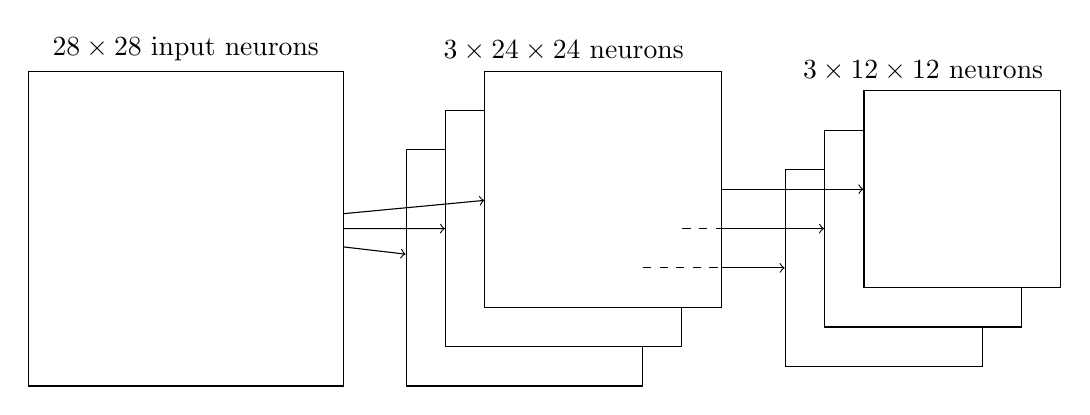
\begin{tikzpicture}[
    inputlayer/.style={rectangle,draw,fill=white,inner sep=0pt,minimum size=40mm},
    hiddenlayer/.style={rectangle,draw,fill=white,inner sep=0pt,minimum size=30mm},
    poolinglayer/.style={rectangle,draw,fill=white,inner sep=0pt,minimum size=25mm}
    ]

    \node (input) [inputlayer,anchor=south west] at (0,0) {};

    \node (hidden0) [hiddenlayer,anchor=south west] at (4.8,0) {};
    \node (hidden1) [hiddenlayer,anchor=south west,xshift=5mm,yshift=5mm] at (hidden0.south west) {};
    \node (hidden2) [hiddenlayer,anchor=south west,xshift=5mm,yshift=5mm] at (hidden1.south west) {};
    
    \foreach \x in {0,1,2}
      \node (pooling\x) [poolinglayer,anchor=west,right=1.8 of hidden\x] {};

    \node [above] at (input.north) {$28 \times 28$ input neurons};
    \node [above,xshift=-5mm] at (hidden2.north) {
      $3 \times 24 \times 24$ neurons
    };
    \node [above,xshift=-5mm] at (pooling2.north) {
      $3 \times 12 \times 12$ neurons
    };

    \foreach \x in {0,...,2}
      \draw[->] (input) to (hidden\x);
      
    \draw[dashed] (hidden0.east) -- ++(10mm,0);
    \draw[->] (hidden0.east)++(10mm,0) -- (pooling0.west);

    \draw[dashed] (hidden1.east) -- ++(5mm,0);
    \draw[->] (hidden1.east)++(5mm,0) -- (pooling1.west);

    \draw[->] (hidden2) to (pooling2);

  \end{tikzpicture} 
\end{document}
